%
% Master thesis template for Ghent University (2021)
%
%
%  !!!!!!!!!!!!!!!!!!!!!!!!!!!!!!!!!!!!!!!!!!!!!!!!!!!!!!!!!!!!
%  !!  MAKE SURE TO SET lualatex OR xelatex AS LATEX ENGINE  !!
%  !!!!!!!!!!!!!!!!!!!!!!!!!!!!!!!!!!!!!!!!!!!!!!!!!!!!!!!!!!!!
%  !! For overleaf:                                          !!
%  !!     1. click gear icon in top right                    !!
%  !!     2. select `lualatex` in "latex engine"             !!
%  !!     3. click "save project settings"                   !!
%  !!                                                        !!
%  !!!!!!!!!!!!!!!!!!!!!!!!!!!!!!!!!!!!!!!!!!!!!!!!!!!!!!!!!!!!
%
%
%  History
%    2014         Doctoral Thesis of Bruno Volckaert
%    2017         Adapted to master thesis by Jerico Moeyersons
%    2018         Cleanup by Merlijn Sebrechts
%    2021         Update by Marleen Denert and Merlijn Sebrechts with feedback from Leen Pollefliet
%    2022         Update by Merlijn Sebrechts
%
%  Latest version
%    https://github.com/galgalesh/masterproef-template
%

% Note: remove `openany` for printed version
\documentclass[11pt,a4paper,openany,dutch,english]{book}
\usepackage[a4paper,includeheadfoot,margin=2.50cm]{geometry}




\renewcommand{\baselinestretch}{1.2}  % stretch horizontal space between everything

\usepackage[hyphens]{url} % Break line on hyphens in long urls
\usepackage{graphicx}
\graphicspath{{images/}}
\usepackage{pdfpages}
\usepackage{enumitem}
\usepackage{float}
\usepackage{caption}
\usepackage{subcaption}
\usepackage[toc,page]{appendix}
\usepackage{fontspec}
\usepackage[T1]{fontenc}

% Don't indent table of contents, list of figures, and list of tables
\usepackage{tocloft}
\setlength{\cftsecindent}{0pt}    % Remove indent for \section in Table of Contents
\setlength{\cftsubsecindent}{0pt} % Remove indent for \subsection in Table of Contents
\setlength{\cftfigindent}{0pt}    % remove indentation from figures in List of Figures
\setlength{\cfttabindent}{0pt}    % remove indentation from tables in List of Tables

\usepackage{parskip} % Add space between two paragraphs and don't indent the first line of the paragraph

% To generate fake lorem ipsum text
\usepackage{lipsum}



%
% UGent style guide
%
\setmainfont[
	Path=fonts/,
	BoldFont      =UGentPannoText-SemiBold.ttf,
	ItalicFont    =UGentPannoText-Normal.ttf,
	ItalicFeatures={FakeSlant=0.3},
	BoldItalicFont=UGentPannoText-SemiBold.ttf,
    BoldItalicFeatures={FakeSlant=0.3},
]{UGentPannoText-Normal.ttf}
\urlstyle{same} % Also use the default font for URLs


% If you want left justified text, uncomment the line below.
%\usepackage[document]{ragged2e} % Left justify all text

% Style Chapter titles so they have the chapter number in grey.
\usepackage{color}
\definecolor{chaptergrey}{rgb}{0.5,0.5,0.5}
\usepackage[explicit, pagestyles]{titlesec}
\titleformat{\chapter}[display]{\bfseries}{\color{chaptergrey}\fontfamily{pbk}\fontsize{80pt}{100pt}\selectfont\thechapter}{0pt}{\Huge #1}
\titlespacing*{\chapter}{0pt}{-80pt}{30pt}


% Header showing chapter number and title and footer showing page number
\newpagestyle{fancy}{%
  \sethead{} % left
          {} % center
          {\Large\thechapter~~\chaptertitle} %right
  \setfoot{} % left
          {\thepage} % center
          {} %right
  \setheadrule{0pt}
}
\pagestyle{fancy}

% Header showing chapter title and footer showing page number
\newpagestyle{numberless}{%
  \sethead{} % left
          {} % center
          {\Large\chaptertitle} %right
  \setfoot{} % left
          {\thepage} % center
          {} %right
  \setheadrule{0pt}
}

% We use the package `minted` for modern code highlighting.
\usepackage[newfloat,chapter]{minted}
\SetupFloatingEnvironment{listing}{name=Codefragment, listname=Lijst van codefragmenten}
%\SetupFloatingEnvironment{listing}{name=Code Fragment, listname=List of Code Fragments} % lang:english


\PassOptionsToPackage{hyphens}{url}
\usepackage{hyperref}
\usepackage{url}

\usepackage[numbers]{natbib}       % For bibliography; use numeric citations
\bibliographystyle{IEEEtran}
\usepackage[nottoc]{tocbibind}     % Put Bibliography in ToC

%
% Defines \checkmark to draw a checkmark
%
\usepackage{tikz}
\def\checkmark{\tikz\fill[scale=0.4](0,.35) -- (.25,0) -- (1,.7) -- (.25,.15) -- cycle;}

%
% For tables
%
\usepackage{booktabs}
\usepackage{array}
\usepackage{ragged2e}  % for '\RaggedRight' macro (allows hyphenation)
\newcolumntype{L}[1]{>{\raggedright\let\newline\\\arraybackslash\hspace{0pt}}m{#1}}
\newcolumntype{C}[1]{>{\centering\let\newline\\\arraybackslash\hspace{0pt}}m{#1}}
\newcolumntype{R}[1]{>{\raggedleft\let\newline\\\arraybackslash\hspace{0pt}}m{#1}}

%
% Support for splitting Dutch words correctly
%
\usepackage{polyglossia}
\setdefaultlanguage[babelshorthands=true]{dutch} % lang:dutch
%\setmainlanguage{english}                       % lang:english

% Manually specify additional hypnations for words
%
% Translated strings. If these aren't set, the English words are used.
%
\addto\captionsenglish{\renewcommand{\contentsname}{Inhoudsopgave}}   % lang:dutch

% Fix error "Package hyperref Warning: The anchor of a bookmark and its parent's must not be the same. Added a new anchor on ..."
\newcommand{\sectionbreak}{\phantomsection}

\renewcommand\appendixtocname{Bijlagen}                     % lang:dutch
\renewcommand\appendixpagename{Bijlagen}                    % lang:dutch


\usepackage[toc,acronym]{glossaries}  % for list of acronyms
\makeglossaries                       % start internal list of acronyms


%
% Set the title and your name
%
%%%%%%%%%%%%%%%%%%%%%%%%%%%%%%%%%%%%%%%%%%%%%%%%%%%%%%%%%%%%%%%%%%%%%%
%
% Add the specific info for your thesis
%
%%%%%%%%%%%%%%%%%%%%%%%%%%%%%%%%%%%%%%%%%%%%%%%%%%%%%%%%%%%%%%%%%%%%%%

\title{Collaborative Compositions: Facilitating Service Orchestration from Cloud to Edge}
\author{Merlijn Sebrechts}







%%%%%%%%%%%%%%%%%%%%%%%%%%%%%%%%%%%%%%%%%%%%%%%%%%%%%
% Add all the acronyms you use in your thesis here. %
% These will be added to the List of Acronyms       %
%%%%%%%%%%%%%%%%%%%%%%%%%%%%%%%%%%%%%%%%%%%%%%%%%%%%%


\newacronym{IP}{IP}{Internet Protocol}
\newacronym{CPU}{CPU}{Central Processing Unit}
\newacronym{vCPU}{vCPU}{Virtual Central Processing Unit}
\newacronym{RAM}{RAM}{Random Access Memory}
\newacronym{TCP}{TCP}{Transmission Control Protocol}
\newacronym{VM}{VM}{Virtual Machine}
\newacronym{IT}{IT}{Information Technology}
\newacronym{API}{API}{Application Programming Interface}
\newacronym{UI}{UI}{User Interface}
\newacronym{GUI}{GUI}{Graphical User Interface}
\newacronym{VPN}{VPN}{Virtual Private Network}
\newacronym{REST}{REST}{Representational State Transfer}
\newacronym{OS}{OS}{Operating System}
\newacronym{HTTP}{HTTP}{HyperText Transfer Protocol}
\newacronym{HTTPS}{HTTPS}{HyperText Transfer Protocol Secure}
\newacronym{SSL}{SSL}{Secure Sockets Layer}
\newacronym{Sysadmins}{sysadmins}{System Administrators}
\newacronym{TOSCA}{TOSCA}{OASIS Topology and Orchestration Specification for Cloud Applications}
\newacronym{ISV}{ISV}{Independent Software Vendors}
\newacronym{M@RT}{M@RT}{Models@run.time}
\newacronym{SA}{SA}{Service Agent}
\newacronym{VNF}{VNF}{Virtual Network Function}
\newacronym{BPMN}{BPMN}{Business Process Modeling Notation}
\newacronym{OA}{OA}{Orchestration Agent}
\newacronym{IoT}{IoT}{Internet of Things}
\newacronym{k8s}{k8s}{Kubernetes}
\newacronym{PaaS}{PaaS}{Platform as a Service}
\newacronym{SSE}{SSE}{Server-Sent Events}
\newacronym{CA}{CA}{Certificate Authority}
\newacronym{CDK}{CDK}{Canonical Distribution of Kubernetes}
\newacronym{DAG}{DAG}{Direct Acyclic Graph}
\newacronym{IQR}{IQR}{Interquartile Range}
\newacronym{QoS}{QoS}{Quality of Service}
\newacronym{Mbps}{Mbps}{Megabits per second}
\newacronym{Km}{Km}{Kilometers}
\newacronym{HnS}{H\&S}{Hub and Spoke}
\newacronym{SLA}{SLA}{Service-Level Agreement}
\newacronym{AWS}{AWS}{Amazon Web Services}
\newacronym{EC2}{EC2}{Elastic Compute Cloud}
\newacronym{FWO}{FWO}{Flemish Fund Scientific Research (Fonds Wetenschappelijk Onderzoek - Vlaanderen)}
\newacronym{VLAIO}{VLAIO}{Flemish Agency for Innovation and Entrepreneurship (Vlaams Agentschap Innoveren en Ondernemen)}
\newacronym{VRT}{VRT}{Flemish Radio and Television (Vlaamse Radio en Televisie)}
\newacronym{SBO}{SBO}{Strategic Basic Research (Strategisch BasisOnderzoek)}
\newacronym{RQ}{RQ}{Research Question}
\newacronym{IEEE}{IEEE}{Institute of Electrical and Electronics Engineers}
\newacronym{SDK}{SDK}{Software Development Kit}
\newacronym{JSON}{JSON}{JavaScript Object Notation}
\newacronym{YAML}{YAML}{Yet Another Markup Language}
\newacronym{ID}{ID}{Identifier}
\newacronym{ISP}{ISP}{Internet Service Provider}
\newacronym{UAV}{UAV}{Unmanned Aerial Vehicle}
\newacronym{STEM}{STEM}{Science, Technology, Engineering and Mathematics}
\newacronym{FSM}{FSM}{Finite State Machine}
\newacronym{ITIL}{ITIL}{Information Technology Infrastructure Library}
\newacronym{CI/CD}{CI/CD}{Continuous Integration and Continuous Deployment}
\newacronym{CD}{CD}{Continuous Deployment}
\newacronym{AIOps}{AIOps}{Artificial Intelligence for IT Operations}



%
%  END OF HEADER
%  The actual latex document content starts here.
%
\begin{document}
\frontmatter
\pagestyle{empty}

% Download the cover sheet from Plato
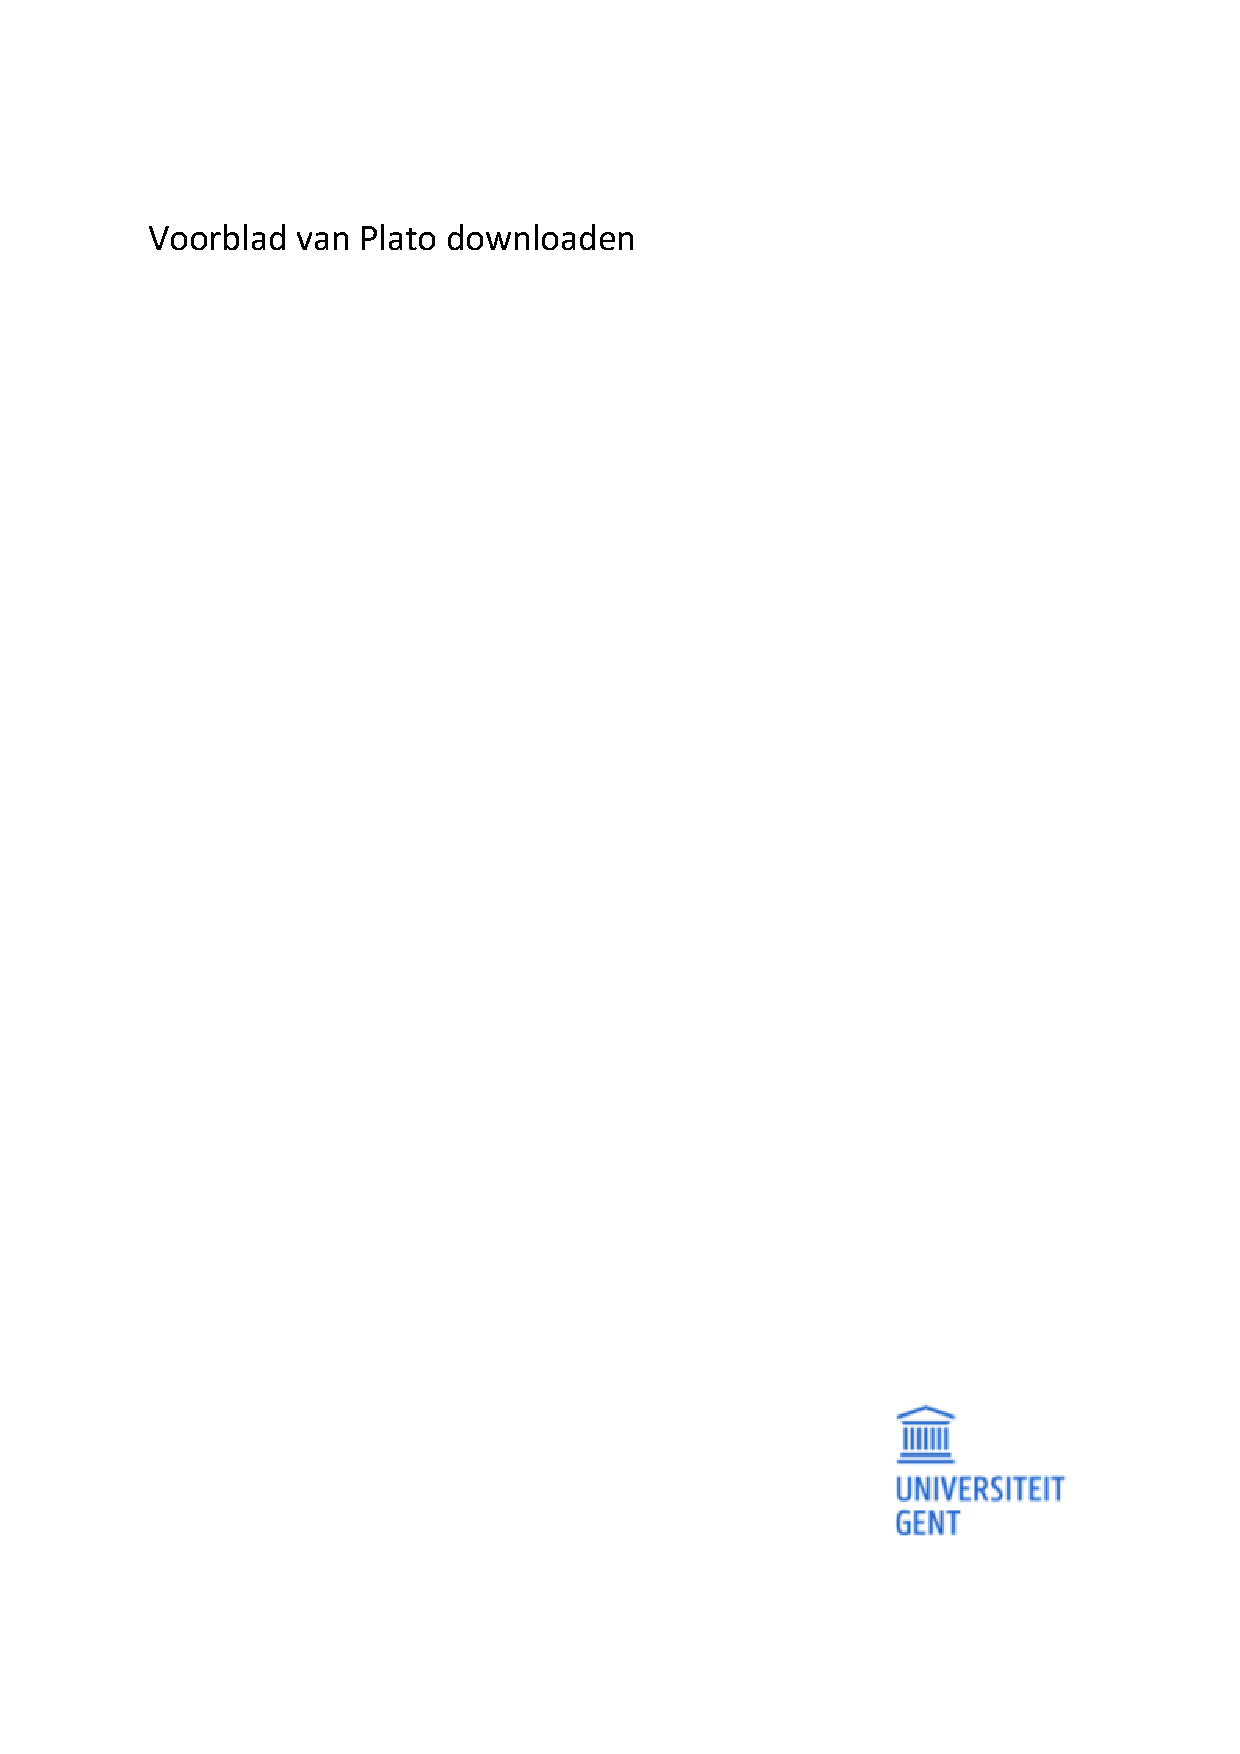
\includepdf{cover-sheet.pdf}

\chapter*{Dankwoord}

\lipsum[2-4]

\chapter*{Toelichting in verband met het masterproefwerk}

Deze masterproef vormt een onderdeel van een examen. Eventuele opmerkingen die door de beoordelingscommissie tijdens de mondelinge uiteenzetting van de masterproef werden geformuleerd, werden niet verwerkt in deze tekst.

% This master's dissertation is part of an exam. Any comments formulated by the assessment committee during the oral presentation of the master's dissertation are not included in this text.

\subsection*{Melding van vertrouwelijkheid (enkel indien van toepassing)}

Bekijk hiervoor de informatie op \href{https://www.ugent.be/ea/nl/faculteit/studentenadministratie/masterproef/} {de facultaire website} - \textbf{Nota in verband met de vorm van de masterproef (alle opleidingen)}
\chapter*{Abstract}
\chaptermark{Abstract}
\addcontentsline{toc}{chapter}{Abstract}  

Meer informatie op \href{https://masterproef.tiwi.ugent.be/verplichte-taken/}{https://masterproef.tiwi.ugent.be/verplichte-taken/} - Korte abstract (Nederlands en/of Engels)

% Write the extended abstract as a separate project using the IEEE conference proceedings template, and include the resulting PDF here in the document. You can find the template on Overleaf: https://www.overleaf.com/latex/templates/ieee-conference-template/grfzhhncsfqn. Voeg dit toe als .pdf
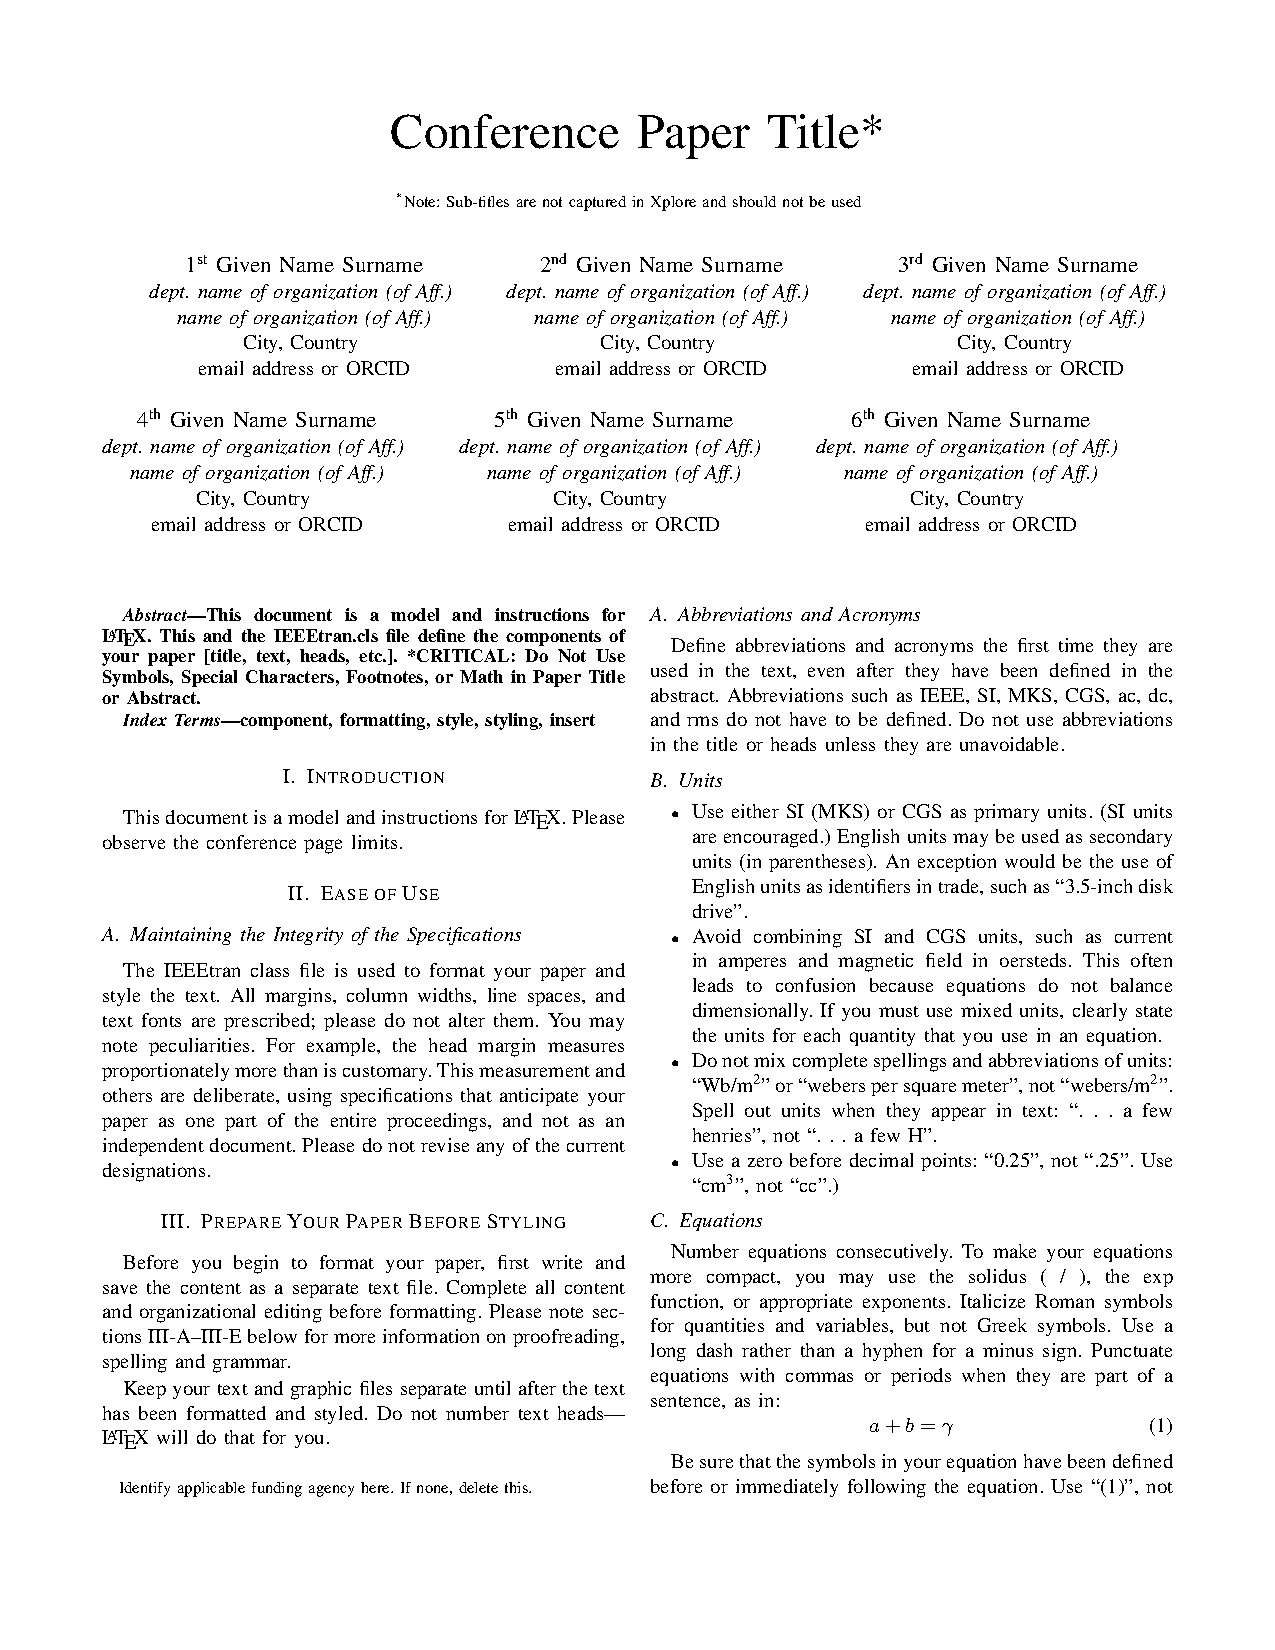
\includepdf[pages={-}]{abstract.pdf}  % Extended Abstract

\tableofcontents\newpage
\listoffigures\newpage
\listoftables\newpage
%%%%%%%%%%%%%%%%%%%%%%%%%%%%%%%%%%%%%%%%%%%%%%%%%%%%%%%%%%%%%%%
%                                                             %
% Note: To add or remove acronyms, modify `personal_data.tex` %
%                                                             %
%%%%%%%%%%%%%%%%%%%%%%%%%%%%%%%%%%%%%%%%%%%%%%%%%%%%%%%%%%%%%%%

\setglossarystyle{listgroup}   % Start from the listgroup style

\setlist[description]{leftmargin=!, labelwidth=10em} % Fixed width for second column
\renewcommand{\glsnamefont}[1]{\textmd{#1}}          % Regular font for acronym

% large letters with spacing
\renewcommand*{\glsgroupheading}[1]{
    \item[\Large{\parbox{\textwidth}{\glsgetgrouptitle{#1}\vspace{2mm}}}]
}

% increase spacing after all acronyms with same initial
\renewcommand*{\glsgroupskip}{
    \vspace{1.5cm}
}

% reduce spacing between acronyms
\renewcommand*{\glspostdescription}{
    \vspace{-0.25cm}
}

% Print the glossary using the new style
\printglossary[type=\acronymtype, title={Lijst van afkortingen}]
%\printglossary[type=\acronymtype, title={List of Acronyms}] % English

\glsaddallunused[\acronymtype]                              % make sure all unused acronyms are in list

\setlist[description]{style=standard} % reset list settings back to default

\listoflistings\newpage

%
% Include the main chapters of the thesis below
% Note: it's best to avoid spaces in filenames as Latex might complain about them.
%
\mainmatter
\pagestyle{fancy} % Use header
\chapter{Inleiding}
\label{chap:intro}

\lipsum[66]

\begin{figure}[h]
	\centering
	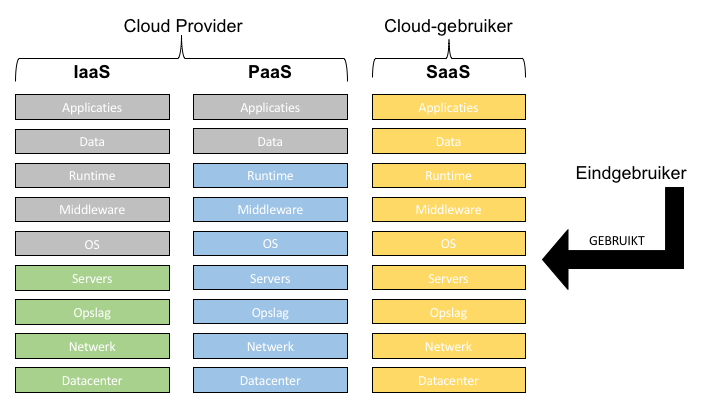
\includegraphics[width=\textwidth]{images/cloud_rollen.png}
	\caption{Image with caption.}
	\label{fig:cloud_rollen}
\end{figure}

\lipsum[67-68]

\begin{listing}[!h]
\begin{minted}[samepage]{js}
alert( 'Hello, world!' );
alert( 'Hello, world!' );
alert( 'Hello, world!' );
alert( 'Hello, world!' );
alert( 'Hello, world!' );
alert( 'Hello, world!' );
alert( 'Hello, world!' );
alert( 'Hello, world!' );
alert( 'Hello, world!' );
alert( 'Hello, world!' );
alert( 'Hello, world!' );
\end{minted}
\caption{Code embedded in document}
\end{listing}

\lipsum[68]

\section{Sectie titel}

In Tabel~\ref{tab:resallocschemes} wordt een overzicht weergegeven ...

\begin{table}[h]
	\centering
	\captionsetup{justification=centering}
	\caption[Overzicht resource-allocatieschema's]{Overzicht resource-allocatieschema's}
	\label{tab:resallocschemes}
	\resizebox{\textwidth}{!}{%
	\begin{tabular}{L{4cm} l C{2cm} c c c c}
		\toprule
		Naam & Jaar & Type  & A | F | P  & Invoer & Uitvoer & Getest  \\ \midrule
		Alicherry et al.~\cite{Alicherry2012} & 2012 & k-sneden & A & G & par\{G\} & S \\
		MCRVMP~\cite{Biran2012} & 2012 & ILP \& GH & A & B\{netwerk\} & VM-plaatsing & C\\
		\bottomrule
	\end{tabular}}
\end{table}

\lipsum[66-68]

Hoofdstuk~\ref{sec:related_work} beschrijft..

\chapter{Titel van het tweede hoofdstuk}
\label{chap:rel_work}

In dit hoofdstuk ...

\section{Sectie titel 1}
\label{sec:related_work}
Vul aan ...
\section{Sectie titel 2}
Vul aan ...
\chapter{Titel derde hoofdstuk}
\label{chap:evaluation}

In dit hoofdstuk ...

\section{Sectie titel}
\label{sec:scalable_faafo}

Vul aan...

\chapter{Titel vierde hoofdstuk}

\lipsum[20]

\lipsum[21-22]

\section{Sectie titel}

\lipsum[32-34]

\section{Sectie titel2}

\lipsum[6-8]


\subsection{Subtitel}

\lipsum[31]

\chapter*{Conclusie}
\chaptermark{Conclusie}
\addcontentsline{toc}{chapter}{Conclusie}  

Vul aan...

\phantomsection
\section*{Ethische en maatschappelijke reflectie}
\addcontentsline{toc}{section}{Ethische en maatschappelijke reflectie}  

Deze sectie is enkel vereist voor de opleidingen industrieel ingenieur. De locatie van deze sectie lichtjes af van de volgorde voorgeschreven door de faculteit. Wij raden aan om deze reflectie als deel van de conclusie te maken omdat je daardoor eenvoudig kan refereren naar resultaten in je masterproef zelf.

Meer informatie kan je opzoeken op https://www.sdgs.be/nl/sdgs




\renewcommand\bibname{Referenties}
\bibliography{referenties}


\pagestyle{numberless} 
\pagestyle{empty}
\begin{appendices}
\section*{Bijlage A}
\addcontentsline{toc}{section}{Bijlage A}  

Toelichting bijlage.



\newpage
\section*{Bijlage B}
\addcontentsline{toc}{section}{Bijlage B}  

Toelichting bijlage.

\end{appendices}


\end{document}
